\chapter{Methodology}
\label{ch:method}

\section{Overview and design principles}
\label{sec:method-overview}

Three decisions shaped this chapter more than any others. Two came from Dr Chen in late July and one from the demonstrator in August, and they are set out before following the data through the chapter in the order it is processed.

The first is that the comparison is one of similarity. Dr Chen's view was that, with emotion subjective, people in disagreement and models noisy, scoring a drawing as a match or a miss against one label would be too crude, and she asked for the similarity framing to be stated as the novel element. Each reader therefore returns a scored list over one set of seven families, and the two lists are compared on four measures arranged as a ladder, from a forgiving circumplex distance up to a strict test of the top family (Section~\ref{sec:method-measures}). All four rungs are reported together.

The second is that no value is quoted without its chance level. This one was not there from the start. While the demonstrator was being wired up in August it became clear that records paired at random already scored around \FullNeuVaNull{} on the loosest measure, since the seven centroids crowd into a small part of the plane and the lowest value the measure can take is 0.412. So 0.71 looks respectable and is under chance. From then on every cell of every table got a random-pairing null (Section~\ref{sec:method-null}); the clustered intervals and the test of the face/scene contrast came later, in the September audits (Section~\ref{sec:method-inference}).

The third is that the vision model is at no point asked about emotion. This too was Dr Chen's instruction, since CLIP learned from colour photographs and is good at objects. The describer answers five plain questions about what is drawn, a fixed template makes one sentence of the answers, and a second text model reads a family out of that sentence, so both sides of the comparison end up as text (Section~\ref{sec:method-pipeline}). How much independence that buys is measured in Section~\ref{sec:method-analyses}, and it is less than expected. Figure~\ref{fig:pipeline} shows the chain.

\begin{figure}[htbp]
\centering
\resizebox{\textwidth}{!}{% TikZ: the describe-then-extract pipeline and the similarity ladder. Input from chapter3.tex.
\begin{tikzpicture}[
  font=\small,
  node distance=6mm and 10mm,
  box/.style={draw, rounded corners=2pt, align=center, minimum height=8mm, inner sep=4pt, fill=white},
  data/.style={box, fill=black!4},
  model/.style={box, fill=blue!8},
  res/.style={box, fill=green!8},
  meas/.style={box, fill=orange!10, minimum width=30mm},
  arr/.style={-{Latex[length=2mm]}, thick},
  lab/.style={font=\scriptsize, text=black!60, yshift=1mm}
]
% prompt lane
\node[data] (prompt) {prompt text\\\footnotesize e.g.\ ``tired but happy''};
\node[model, right=of prompt] (goe) {prompt reader\\\footnotesize GoEmotions, 28 labels};
\node[res, right=of goe] (pfam) {top-3 families\\\footnotesize $P$};
\draw[arr] (prompt) -- (goe);
\draw[arr] (goe) -- node[lab, above] {28 $\to$ 7} (pfam);

% image lane
\node[data, below=14mm of prompt] (img) {line drawing};
\node[model, right=of img] (vqa) {describer\\\footnotesize BLIP-VQA, five factual questions};
\node[data, right=of vqa] (desc) {one-sentence\\description};
\node[model, right=of desc] (nli) {image reader\\\footnotesize BART-MNLI, zero-shot};
\node[res, right=of nli] (ifam) {top-3 families\\\footnotesize $Q$};
\draw[arr] (img) -- (vqa);
\draw[arr] (vqa) -- node[lab, above] {template} (desc);
\draw[arr] (desc) -- node[lab, above] {entailment} (nli);
\draw[arr] (nli) -- (ifam);

% ladder
\node[meas, below=16mm of desc, xshift=-12mm] (va) {valence--arousal similarity};
\node[meas, right=3mm of va] (sign) {valence-sign agreement};
\node[meas, right=3mm of sign] (fam) {family agreement};
\node[meas, right=3mm of fam] (ovl) {top-3 soft overlap};
\node[draw, dashed, rounded corners, inner sep=3pt, fit=(va)(sign)(fam)(ovl), label={[lab]above left:similarity ladder: four measures}] (ladder) {};
\draw[arr] (pfam.east) -- ++(6mm,0) |- ($(ladder.north east)+(0,2mm)$) -- (ladder.north east);
\draw[arr] (ifam.south) -- (ladder.north -| ifam.south);

% null
\node[box, fill=red!6, below=6mm of ladder, text width=110mm] (null) {random-pairing null: re-pair $Q$ with $P$ at random $K$ times $\to$ mean, sd $\to$ $z$\\\footnotesize degenerate (sd $=0$) $\Rightarrow$ no $z$; intervals and tests cluster on the prompt group};
\draw[arr] (ladder) -- (null);
\end{tikzpicture}
}
\caption{The chain from prompt and drawing to the four measures. Top: the prompt reader turns the visitor's words into three scored families. Middle: the describer answers five questions, the template makes one sentence of the answers, and the image reader scores the seven families by entailment. Bottom: the four measures and the random-pairing null that each of them is compared with; a null with zero spread yields no $z$, and every interval and test clusters on the prompt group.}
\label{fig:pipeline}
\end{figure}

\section{The corpus}
\label{sec:method-corpus}

The data are \nTotal{} records from Sheffield's Festival of the Mind in September 2024. Visitors typed how they felt. The box accepted any text, and each entry produced one drawing for the visitor to look at. Every drawing is monochrome line art, 1024 by 1024 pixels, because the installation software added a style instruction to every prompt, and the instruction itself was not passed on with the data. What arrived was one JSON file of \nTotal{} bare strings keyed by position, no labels, no metadata, no participant identifiers, plus a folder of \nTotal{} PNG files whose only link to the strings is their order.

Each PNG also carries a C2PA (Coalition for Content Provenance and Authenticity) provenance manifest. It names DALL$\cdot$E as the software agent, without a version, and holds no seed and no copy of the rewritten prompt that DALL$\cdot$E composes before it draws \cite{betker2023improving}, so nothing can be regenerated and the generation settings are unknown. Its signing time, though, did a lot of work in the pre-processing (Section~\ref{sec:method-preprocessing}).

Most prompts are short. Half of them have four words or fewer, the mean is about six, the longest runs to 107 words, and 294 of the analysed prompts consist of one word (Figure~\ref{fig:promptlength}). About 78\% never use a capital letter, and a handful are written in Italian, in French or in German. The commonest entry is ``happy'', drawn \nHappy{} times. Mixed feelings are common (``tired proud happy'', ``tired but happy''), and a fair number of entries are not about feelings at all: objects (``pigs''), pop culture (``mickey mouse''), questions put to the machine, place names.

Records are not people. Among the \nAnalysed{} analysed records, \nRepeats{} are repeats of a prompt someone had already typed, so how many people took part is unknown, \nDistinct{} is the upper bound, and any interval that treats records as independent will be too narrow (Section~\ref{sec:method-inference}). Figure~\ref{fig:dataset} gives the make-up of the corpus after pre-processing: \nPretest{} tests set aside, then the prompt reader's split (\nEmotional{} emotional, \nNonEmotional{} neutral-labelled) and, within the emotional prompts, the describer's (\nFaceEmo{} face-classified, \nSceneEmo{} scene-classified).

\begin{figure}[htbp]
\centering
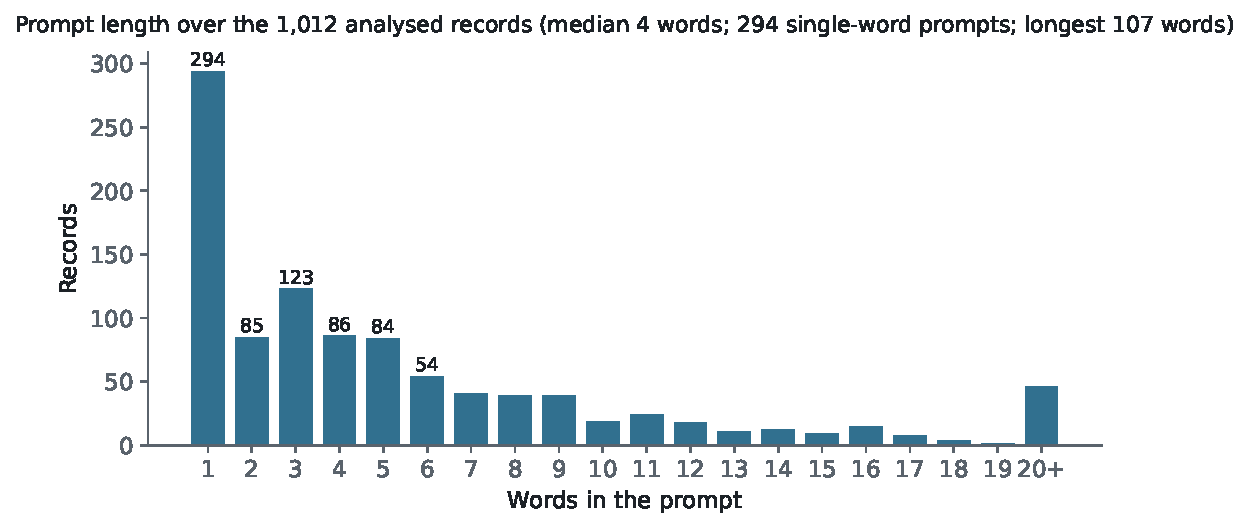
\includegraphics[width=\textwidth]{fig_prompt_length}
\caption{Word counts of the \nAnalysed{} analysed prompts, with the tail collapsed at twenty words: median four words, 294 prompts of one word, longest 107 words.}
\label{fig:promptlength}
\end{figure}

\begin{figure}[htbp]
\centering
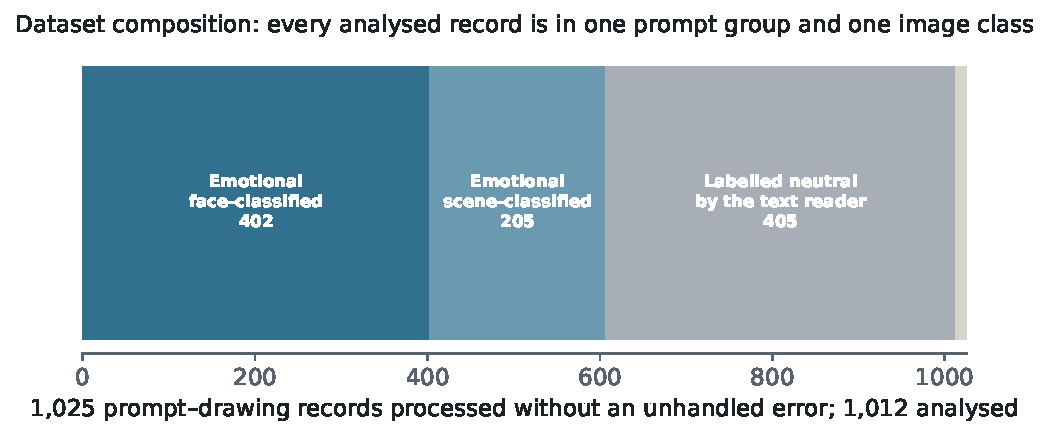
\includegraphics[width=\textwidth]{fig5_dataset}
\caption{What the \nTotal{} records became after pre-processing: \nPretest{} pre-festival tests set aside, then the \nAnalysed{} analysed records divided by the prompt reader into emotional and neutral-labelled prompts and, within the emotional prompts, by the describer into face-classified drawings and scene-classified ones. These are groupings for analysis; no analysed record is excluded by them.}
\label{fig:dataset}
\end{figure}


\section{Data pre-processing}
\label{sec:method-preprocessing}

\subsection{Loading and pre-test removal}

Nothing could be analysed until the files could be opened. Three naming patterns share one directory. The earliest records are zero-padded (\texttt{img\_00001.PNG}), the middle block is unpadded (\texttt{img\_200.PNG}), the records from 1000 onwards have a \texttt{t} before the number (\texttt{img\_t1000.PNG}), and records 2 and 4 end in lower-case \texttt{.png}, which a case-sensitive file system reads as another name. A loader written for the first pattern finds fewer than one file in five. \texttt{emoviz/data.py} handles all three and asserts that exactly \nTotal{} records resolve, so a missing file stops the run instead of quietly shrinking the sample.

The timestamps came out of the same loader. Every C2PA manifest carries an RFC-3161 signing time, and reading it gave each image a date the supplied files did not expose (Figure~\ref{fig:timeline}). The first \nPretest{} records date from 26 August to 18 September 2024, before the festival opened, on scattered days, as a developer testing the installation would, so they are excluded from every analysis and pushed through the pipeline all the same, so that the completion count covers everything. All the others up to the penultimate record fall on 19--29 September 2024, with none on 23 September. The last record, signed on 20 October 2024, is kept.

\begin{figure}[htbp]
\centering
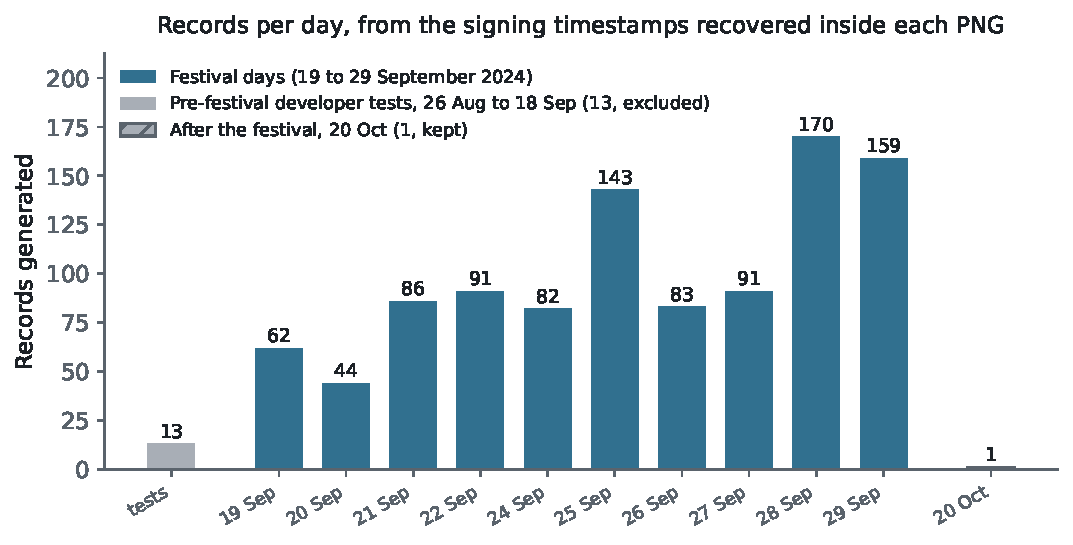
\includegraphics[width=\textwidth]{fig_timeline}
\caption{Records per day from the signing timestamps inside the PNG files. The \nPretest{} developer tests from 26 August to 18 September 2024 are shown apart on the left; the festival days run from 19 to 29 September with none on 23 September; the single record signed on 20 October is on the right and is kept.}
\label{fig:timeline}
\end{figure}

\subsection{Prompt groups}

Each record belongs to one prompt group. The group identifier is the prompt with surrounding whitespace removed and case folded. There are \nDistinct{} groups. \nGroups{} contain more than one record, those hold \nGroupRecords{} records, and \nPairGroups{} are pairs. The identifier is computed from the text as typed, before any name is redacted, and that order matters, because two different names collapse to one placeholder and an identifier computed after redaction would merge two unrelated prompts (this went wrong once in development, and the accounting test caught it). The identifier ignores case but the prompt reader did not, so a few groups hold two slightly different readings (``Ok'' and ``ok'' share one); no count changes because of it.

\subsection{Name redaction}

Eight prompts name a private individual, a friend, a relative, a teacher. Dr Chen's direction at the end of July was to handle this as data pre-processing, replacing the name of a private person with a placeholder while leaving in what visitors wrote about illness, grief and hard times, since that content identifies nobody on its own and the analysis needs it. Redaction runs at load time. The files on disk stay as they were, and analysis, figures and demonstrator all read the same redacted text.

The procedure has three stages, each written up in Appendix~\ref{app:instruments}. Detection favours recall. Since so few visitors used capitals, three detectors run together, an NLTK list of 7,944 given names \cite{bird2009natural}, capitalised tokens in mid-sentence that are missing from an English word list of 236,000 entries, and phrases of the form ``called X'' or ``my friend X''. Review attaches a decision, keep or redact, and a reason to every candidate and ties each redaction to one record, so that ``Jack Frost'' and ``woolly mammoth'' stay as they are. The audit refuses to pass while any candidate is undecided or any redaction entry has nothing left to act on. Application then swaps the token and merges adjacent placeholders.

Running the prompt reader again on the redacted text moved every family probability by 0.012 or less and left every top-1 family where it was, so every analysis uses the same prompt labels with or without the placeholder. Two entries were nothing but a name. They reduce to the bare placeholder (\CtrlNameOnly{} records), and the control audit (Section~\ref{sec:method-analyses}) confirms that they make no difference there either. The decision table names the tokens it removes, so it is kept with the dataset and out of the code folder.

\section{The pipeline}
\label{sec:method-pipeline}

\subsection{Prompt reader}

The prompt reader is RoBERTa fine-tuned on GoEmotions \cite{demszky2020goemotions}, the \texttt{SamLowe/\allowbreak roberta-base-go\_emotions} checkpoint, roughly 125 million parameters. Its output is 28 probabilities, one per category. These are added up into the seven families the GoEmotions authors proposed (Appendix~\ref{app:instruments}), the seven sums are rescaled so that they add to one, and the top three are kept as the prompt reading. A prompt counts as emotional whenever its top family is anything other than neutral, which makes \nEmotional{} of the \nAnalysed{} analysed prompts emotional and \nNonEmotional{} neutral-labelled. Nobody checked those labels. They are the reader's opinion, so the neutral-labelled prompts are kept as a group of their own and audited (Section~\ref{sec:method-analyses}).

GoEmotions was the third reader tried on this side. My first pipeline used a hand-built lexicon, transparent but unable to represent ``calm but tired'' except by letting one word win, and the prompts are full of blends like that. The same NLI model was then put on both sides. On short prompts it over-read surprise. Roughly a third of the corpus was labelled surprise in that run, the hypothesis wording misfiring on two-word inputs. GoEmotions has no such artefact. It was trained on Reddit comments written in the first person, as close to a festival entry as training data gets, and swapping it in left every headline result where it was.

\subsection{Describer}

The describer is BLIP-VQA \cite{li2022blip}, the \texttt{Salesforce/blip-vqa-base} checkpoint, roughly 385 million parameters. It gets five fixed questions per drawing. They always come in the same order, expression first, then action, posture, people count and scene (Appendix~\ref{app:instruments}), and none of the five contains the word ``emotion'', in keeping with the third principle above. The answers are cached record by record, so the template ablation can later repeat the extraction stage without touching the vision model at all.

BLIP-VQA is what remained after three attempts that went nowhere. The intended describer was Qwen2.5-VL, a vision--language model of 3 billion parameters, and on the 16~GB laptop available it filled the memory, swapped for 4~h~45~min and completed nothing. Florence-2 came next. It failed on the pinned Transformers 5.14 over a \texttt{forced\_bos\_token\_id} incompatibility. The plain captioning head of BLIP was tried next, but its captions were so terse that the image reader put almost every drawing into one family, surprise. With BLIP-VQA the full run over the \nTotal{} images completed, at between roughly 1 and 12 seconds a record, slowing when memory was short.

\subsection{Description template and image reader}

The five answers become one sentence. The template puts the people count and the scene first, ``A drawing of \{people\} showing \{scene\}.'', then the action and the posture, ``The person is \{action\}, \{posture\}.'', and last of all ``The facial expression is \{expression\}.'' (Appendix~\ref{app:instruments}). That sentence goes to BART fine-tuned on MultiNLI \cite{lewis2020bart, williams2018broad}, the \texttt{facebook/bart-large-mnli} checkpoint, roughly 407 million parameters, which scores, for each family, the hypothesis string ``This scene conveys \{family\}'' by entailment in the zero-shot manner of Yin and colleagues \cite{yin2019benchmarking}. The three best-scoring families form the image reading.

One property of the template matters later. The template states, for every record, that there is a person and that the person has a facial expression, even where the describer's own answer to the people question was zero, so a mountain reaches the reader with a person and a facial expression attached. It was written in week one. Nobody measured what that did until the audits in September (Sections~\ref{sec:results-describer} and \ref{sec:results-ablation}). GoEmotions, the one other reader tried on this side, put almost everything in neutral with nearly all the probability on that family, because it wants feeling words in the first person, which a description of a drawing never has.

\subsection{Face and scene classes}

Dr Chen expected faces to be easier than scenes for any reader and asked for the split. The rule is mechanical. Face-classified means two things are true of the describer's answers, that the people count is at least one and that the expression answer contains, as a whole token, one of the readable expression words in Appendix~\ref{app:instruments}, so ``man is smiling'' qualifies. Everything else is scene-classified. A digit or a number word in the people answer gives the count. Over all \nAnalysed{} analysed records the split is \nFaceAll{} to \nSceneAll{}, and inside the emotional prompts it is \nFaceEmo{} to \nSceneEmo{}. The rule was tightened on 1 September, after the first audit, so that only whole tokens count.

The split is partly circular. The class comes out of the describer's answers, and the image reader reads a sentence built from those same answers, which makes part of the face/scene contrast a contrast between two kinds of description. Chapter~\ref{ch:results} puts a number on it. The single-coder check, where a sample of drawings is classed by a person who has not seen the describer's answers, is the only place it is broken.

\section{The similarity ladder}
\label{sec:method-measures}

Each reader returns three families with scores, $T = \{(\ell_i, s_i)\}_{i=1}^{3}$ with $\ell_i \in \mathcal{F}$ and $\mathcal{F} = \{\text{joy}, \text{sadness}, \text{anger}, \text{fear}, \text{surprise}, \text{disgust}, \text{neutral}\}$. $P$ is the prompt reader's list, $Q$ the image reader's; $\operatorname{top}(T) = \ell_1$ is the top family. Each family also has $c_\ell = (v_\ell, a_\ell)$, a fixed point on the valence--arousal plane (Appendix~\ref{app:instruments}). They were placed by hand from the usual positions of the basic emotions on Russell's circumplex \cite{russell1980circumplex}; per-family averages of the NRC valence and arousal norms \cite{mohammad2018obtaining} are the documented alternative, left for further work. The four measures are defined below, beginning with the loosest.

\paragraph{Valence--arousal similarity.} A reading is first reduced to one point on the plane, its score-weighted centroid, and two readings are compared by the distance between their points:
\begin{equation}
\mathbf{v}(T) = \frac{\sum_i s_i\, c_{\ell_i}}{\sum_i s_i}, \qquad
S_{\mathrm{VA}}(P, Q) = 1 - \frac{1}{\sqrt{2}}\,\Bigl\|\Bigl(\tfrac{v_P + 1}{2} - \tfrac{v_Q + 1}{2},\; a_P - a_Q\Bigr)\Bigr\|_2 ,
\label{eq:va}
\end{equation}
Here $(v_P, a_P)$ is $\mathbf{v}(P)$, likewise for $Q$, and valence is mapped onto $[0,1]$ so the two axes span the same range. This rung forgives. A prompt read as joy against a drawing read as surprise scores well here, since the two points lie near each other, although the top families differ. The minimum over the seven fixed points is $0.412$ (joy paired with sadness), and random pairings already average about \FullNeuVaNull{}, so this measure is never reported without its null beside it.

\paragraph{Top-3 soft overlap.} The two readers score on different scales, so each side is rescaled so that its three scores sum to one, $\tilde{p}_\ell = s_\ell / \sum_j s_j$, and the overlap adds up, family by family, the smaller of the two shares,
\begin{equation}
S_{\mathrm{ovl}}(P, Q) = \sum_{\ell \in \mathcal{F}} \min\bigl(\tilde{p}_\ell,\; \tilde{q}_\ell\bigr) \in [0, 1],
\label{eq:overlap}
\end{equation}
It equals one exactly when the two sides coincide. Credit goes to a second or third family that both readers listed, which the top rung ignores, and of the four rungs this is the only one that uses the scores as well as the labels.

\paragraph{Family agreement.} For $n$ records the rate is
\begin{equation}
A_{\mathrm{fam}} = \frac{1}{n} \sum_{i=1}^{n} \mathbb{1}\bigl[\operatorname{top}(P_i) = \operatorname{top}(Q_i)\bigr].
\label{eq:family}
\end{equation}
Of the four this is the least forgiving, and it is the one other studies most often report. Its chance level depends on the marginals. A reader that answers joy for many drawings will agree by accident with a prompt reader that answers joy for many prompts, and Table~\ref{tab:families} shows that both readers here do exactly that.

\paragraph{Valence-sign agreement.} Let $\sigma(\ell) \in \{+, -, 0\}$ map joy to $+$, surprise and neutral to $0$, and the other four families to $-$. Then
\begin{equation}
A_{\mathrm{sign}} = \frac{\sum_{i} \mathbb{1}\bigl[\sigma(\operatorname{top} P_i) \neq 0 \;\wedge\; \sigma(\operatorname{top} P_i) = \sigma(\operatorname{top} Q_i)\bigr]}{\sum_{i} \mathbb{1}\bigl[\sigma(\operatorname{top} P_i) \neq 0\bigr]} ,
\label{eq:sign}
\end{equation}
so a record with an unsigned prompt family drops out of the denominator, and the denominator is printed beside every value it produces; for the emotional prompts it is \FullEmoNSign{} of \FullEmoN{}. It asks the coarsest question there is, whether both readers gave the same sign, and the headline result rests on it.

\section{The random-pairing null}
\label{sec:method-null}

None of the measures starts at zero. Equation~\ref{eq:va} is bounded below, and both readers say joy so often (Table~\ref{tab:families}) that top-1 agreement happens by accident. So every value is compared with the same measure after the image readings have been shuffled against the prompts, the exchangeability hypothesis \cite{good2005permutation}: if a drawing's reading has nothing to do with its prompt, handing each prompt somebody else's drawing changes the measure only by noise. For any subset of $n$ records and any measure $m$, the image side is permuted $K$ times, $\pi_k$ being the $k$-th permutation, and $m_k$ is the measure recomputed on the pairs $(P_i, Q_{\pi_k(i)})$; with $\hat\mu = \frac{1}{K}\sum_k m_k$ the mean of these values and $\hat\sigma$ their standard deviation,
\begin{equation}
z = \frac{m_{\mathrm{obs}} - \hat\mu}{\hat\sigma}, \qquad K = \nullShuffles,\ \text{seed}\ \nullSeed .
\label{eq:z}
\end{equation}

There are two cautions on $z$. First, \nullShuffles{} re-pairings give a rough estimate of the standard deviation in the denominator. Re-running with seeds 1 to 5 puts the headline valence-sign $z$ anywhere from \ZSeedMin{} to \ZSeedMax{} (the null mean moves by under a tenth of a point). $z$ is therefore used to rank effects and never as an exact probability. Second, a null can be degenerate. When a subset's prompts all have the same top family, shuffling the drawings leaves family agreement exactly where it was, and likewise for the sign when every prompt has the same sign; $\hat\sigma$ comes out at zero and $z$ is undefined. The scripts spot this from the spread of the null itself and print nothing in that cell. Before that, two subsets had been flagged by hand and a third missed.

\section{Inference}
\label{sec:method-inference}

Records are not independent, and for a while they were analysed as if they were. \nRepeats{} records share their prompt with an earlier one, and all the drawings of one prompt inherit whatever that prompt does to each reader. The face/scene permutation test and the interval on that difference were run just before the presentation on 4 September; everything else here, the clustered intervals for every other cell, Cohen's kappa, the Holm correction and the paired tests for the two image readers, was added in the second audit on 9 September, when the marking criteria were revisited. The unit of resampling throughout is the prompt group \cite{cameron2008bootstrap}.

\paragraph{Clustered bootstrap intervals.} Let $\mathcal{G}$ be the prompt groups in a subset. One draw takes $|\mathcal{G}|$ groups with replacement, pools every record of the groups it drew and recomputes the measure, and the interval is the middle 95\% of the $B$ bootstrap values \cite{efron1993introduction}, $B = \DiffDraws{}$, seed \nullSeed{}. A group drawn twice counts twice, so a prompt drawn \nHappy{} times moves the interval as one piece of evidence and never as \nHappy{}.

\paragraph{Clustered permutation test of the face/scene difference.} Under the null the image class has no bearing on agreement, so face/scene labels can be shuffled over prompt groups. That is done $P$ times, recomputing the difference each time and counting how often the shuffled difference is at least as extreme as the real one; the two-sided $p$-value follows North and colleagues \cite{north2002note},
\begin{equation}
p = \frac{k + 1}{P + 1}, \qquad k = \#\{\text{permuted differences at least as extreme as the observed}\},
\label{eq:permp}
\end{equation}
With $P = \DiffDraws$ the smallest value that can come out is $10^{-4}$.

\paragraph{Cohen's kappa.} Family agreement is also given as Cohen's kappa, for comparison with other studies,
\begin{equation}
\kappa = \frac{p_o - p_e}{1 - p_e},
\label{eq:kappa}
\end{equation}
Here $p_o$ is the top-1 rate actually observed and $p_e$ the rate the two readers' family marginals would produce on their own if the readers had nothing to do with each other \cite{cohen1960coefficient}. Landis and Koch's bands \cite{landis1977measurement} give the words for it. The interval is the same clustered bootstrap.

\paragraph{Multiple comparisons.} \HolmM{} $z$-scores survive the degeneracy filter. Each becomes a two-sided $p$-value under the normal approximation, and Holm's step-down procedure \cite{holm1979simple} controls the family-wise rate: with the $p$-values sorted, $p_{(1)} \le \dots \le p_{(m)}$, rejection proceeds in order and stops at the first $p_{(i)} > \alpha / (m - i + 1)$, at $\alpha = 0.05$. For the largest $z$ the normal approximation is only nominal, and no decision changes because of it.

\paragraph{Paired comparison of two image readers.} Each record gives each reader a yes or a no. The comparison is therefore paired. Let $b$ be the number of records where only the first reader agrees and $c$ the number where only the second does. McNemar's exact test \cite{mcnemar1947note} on $(b, c)$ assumes independent records and is therefore optimistic here, so a clustered alternative sums the differences inside each prompt group and flips the sign of whole groups at random, \McClusterDraws{} times; the interval on the rate difference is again a clustered bootstrap.

\paragraph{Wilson intervals.} The single-coder check produces proportions from a small sample, some of them near 0 or 1, so they get Wilson score intervals \cite{wilson1927probable}, which behave where the normal interval breaks down.

\section{Analyses}
\label{sec:method-analyses}

The list below follows the order of Chapter~\ref{ch:results}. Each analysis is one script writing one JSON file, and every table, figure and number in the text is generated from those files (Appendix~\ref{app:repro}).

\paragraph{Splits and the main table.} \texttt{analysis\_final.py} produces the main table, four measures each with its null, for the emotional prompts, for the face-classified and the scene-classified records inside them, for the positive and the negative prompts, and for the neutral-labelled prompts, all by Equation~\ref{eq:z}. Only valence--arousal similarity has a live null in the single-valence cells. The same script repeats the table on distinct prompts only, keeping the first record of each of the \nDistinct{} groups, and that is the robustness check for repeated prompts.

\paragraph{The face/scene difference.} \texttt{significance.py} runs the permutation test and the bootstrap interval for the difference, for valence sign and for family. Then \texttt{inference.py} supplies the intervals for the remaining cells, kappa for the emotional, face and scene cells, the Holm step-down over the printed $z$-scores, and the seed check.

\paragraph{Specificity check.} Neutral-labelled prompts are the specificity check: their agreement should sit at the null. Only valence--arousal similarity can be read there, since on a subset with one prompt label the other three nulls have no spread, and the analysis reports the degeneracy in place of a $z$.

\paragraph{Method comparison.} \texttt{method\_comparison.py} changes the image reader and nothing else, with an identical prompt reader, identical records (\McN{} of them), identical measures and identical re-pairings. The second reader is direct CLIP \cite{radford2021learning, ilharco2021openclip}. It is OpenCLIP ViT-B/32 with LAION-2B weights, given the seven family names as text prompts, and its readings sit frozen in a file the main pipeline cannot overwrite. A first-build comparison had used NLI on the prompt side, another subset and another overlap formula, and the first audit on 1 September found its direct-CLIP overlap computed over the wrong label space. Table~\ref{tab:methodvone} keeps it as a record only; the like-for-like version dates from 9 September.

\paragraph{Consistency across repeated prompts.} For a repeat group $g$ of $n_g \ge 2$ records, write $c_g = \max_{\ell} n_{g,\ell} / n_g$ for the share of its drawings given the group's commonest image family. The consistency $C$ is the mean of $c_g$ over the \nGroups{} groups. A pair cannot score under $0.5$, and \nPairGroups{} groups are pairs, so the null shuffles image families over all \nAnalysed{} analysed records, keeps the group boundaries where they are and recomputes $C$, \ConsDraws{} times, and the number of groups with $c_g = 1$ gets the same treatment. The scripted null is a 9 September addition. $C$ bounds the reproducibility of prompt, generator and reader together; it cannot isolate the generator, whose settings were never recorded, and one visitor entering ``happy'' twice looks identical to two visitors entering it once each.

\paragraph{Per-family agreement.} \texttt{audits.py} also breaks family agreement down by prompt family, as the fraction of each prompt family's records that the image reader put in the same family, with clustered intervals; Table~\ref{tab:confusion} has the full cross-tabulation.

\paragraph{Control audit.} The same script scans the \CtrlN{} neutral-labelled prompts for any of \CtrlLexicon{} ordinary affect words, and it picks out the \CtrlNameOnly{} records that redaction reduced to the bare placeholder. The specificity check is then re-run without either set.

\paragraph{Describer audit and copy rate.} The describer's people count is tabulated against whether an expression word is present, and the smile answers are counted with their denominators. The copy rate concerns one-word expression answers. It is the fraction of those records on which the image reader's top family coincides with the family of that word; the strict version admits only words that name a feeling (happy, sad, angry and the like, \DescBareStrictN{} records) and the broad version adds facial actions such as smile and crying (\DescBareBroadN{} records).

\paragraph{Error taxonomy.} \texttt{error\_taxonomy.py} collects the emotional records on which the two readers disagree about the top family while each gives its own top family a score of at least 0.8. Fewer than the intended 40 qualified, so all were examined. An automatic tagger first marks each record (people count, bare expression word, short prompt, ambiguous raw label, connective), and then every drawing was opened and one primary failure mode chosen out of six fixed ones: (a) an invented face or expression, (b) a misread one, (c) a fair description the reader mis-inferred from, (d) a mixed or ambiguous prompt, (e) a drawing unrelated to its prompt, and (f) a prompt the prompt reader mislabelled. A fixed tie-break rule, printed with the counts, settled records where more than one applied.

\paragraph{Template ablation.} \texttt{ablate\_nli.py} takes the cached answers, builds each description again with a modified template, sends only that sentence back through the image reader, and then computes the ladder and the nulls exactly as the main analysis does, seed included. There are five single-clause deletions (expression, action, posture, people, scene), one variant that sets every expression to ``unclear'', and two people-aware variants that shorten the sentence for records with a zero people count, one keeping the action and posture clauses and one keeping only the scene clause. A control run with the original template separates numerical noise from real template effects. It changed \AblControlChanged{} top-1 readings.

\paragraph{Single-coder check.} \texttt{human\_check.py} draws the sample and scores the coding. The sample is 120 drawings chosen by seed in three strata defined by the describer's output, 40 from the face-classified records, 40 from scene-classified records with a zero people count, and every record whose people answer was vague or a single word, the remainder split equally between the first two strata. Six numbered contact sheets hold the drawings and nothing else. The author is the coder, filling the four columns in Appendix~\ref{app:instruments} blind to prompt, description and readings. Once coded, the script scores the people count and the precision and recall of the face rule, both against the coder, what lies behind the ``smiling'' answers, and the coder's valence against the image reader's, with Wilson intervals, and then recomputes the face/scene difference on the coder's classification, the one estimate free of the describer's split. The coding was not finished at the time of writing. Figure~\ref{fig:codingsheet} shows the first sheet.

\begin{figure}[htbp]
\centering
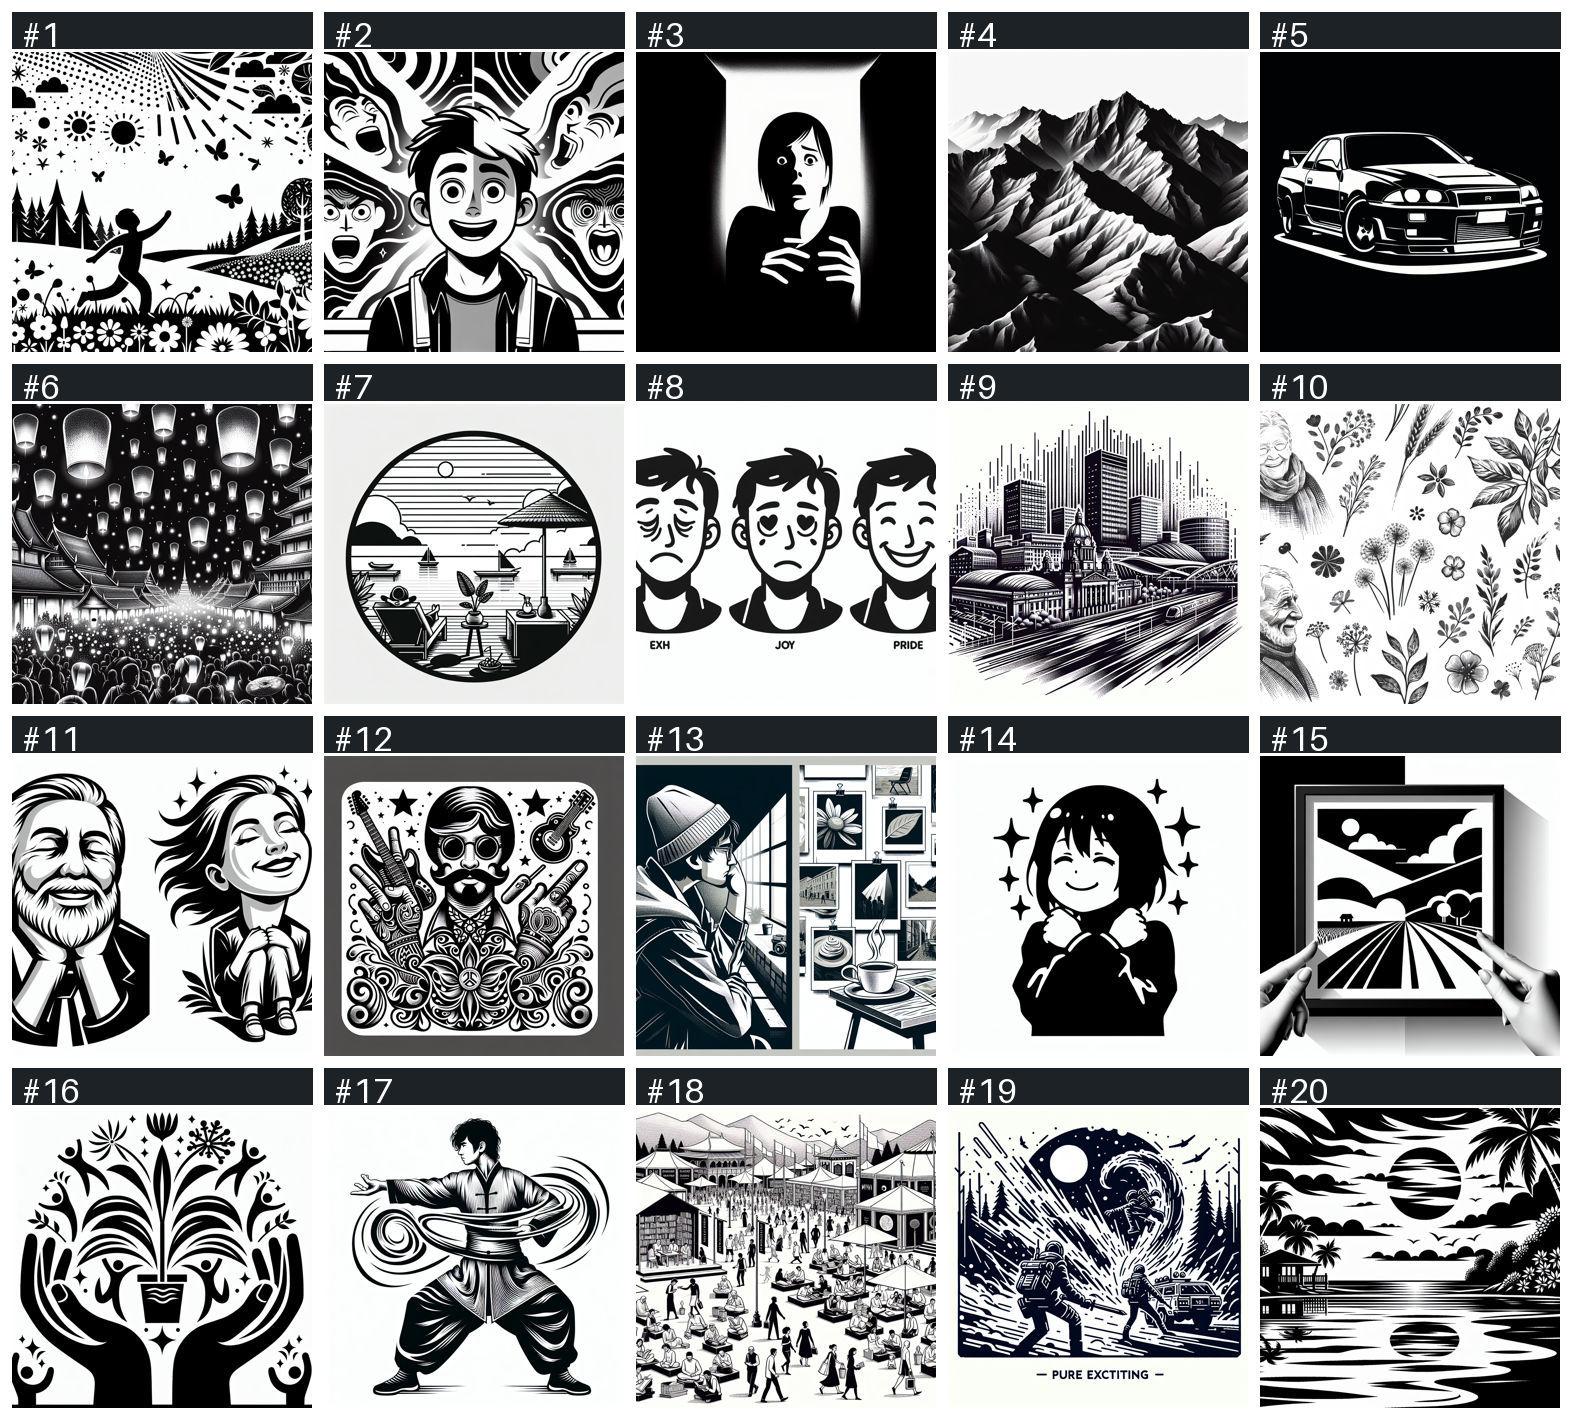
\includegraphics[width=0.9\textwidth]{coding_sheet}
\caption{The first of the six contact sheets for the single-coder check. Only the drawings and their sheet numbers are shown; the prompt, the description and both readings stay hidden until the coding file is complete.}
\label{fig:codingsheet}
\end{figure}

\section{The demonstrator}
\label{sec:method-demo}

The pipeline also runs as a local Flask application, \texttt{app.py} with one page in \texttt{web/index.html}, on port 5050. It applies the real models to any analysed record or an uploaded image and shows the five answers, the sentence built from them, both readings, and the four measures against the null the analysis used, computed when the server starts from the result files. Three choices in the interface come straight from the methodology. The axis for valence--arousal similarity begins at 0.412, its floor, and the middle half of the random pairings is shaded across it, so a below-chance value sits visibly under the band. The verdict puts valence sign and family first and gives the loosest measure only as a percentile among the random pairings. A degenerate chance level is named as degenerate, with no number. The page stores nothing that is typed or uploaded, the request log is switched off, and it was never used to collect data.

\begin{figure}[htbp]
\centering
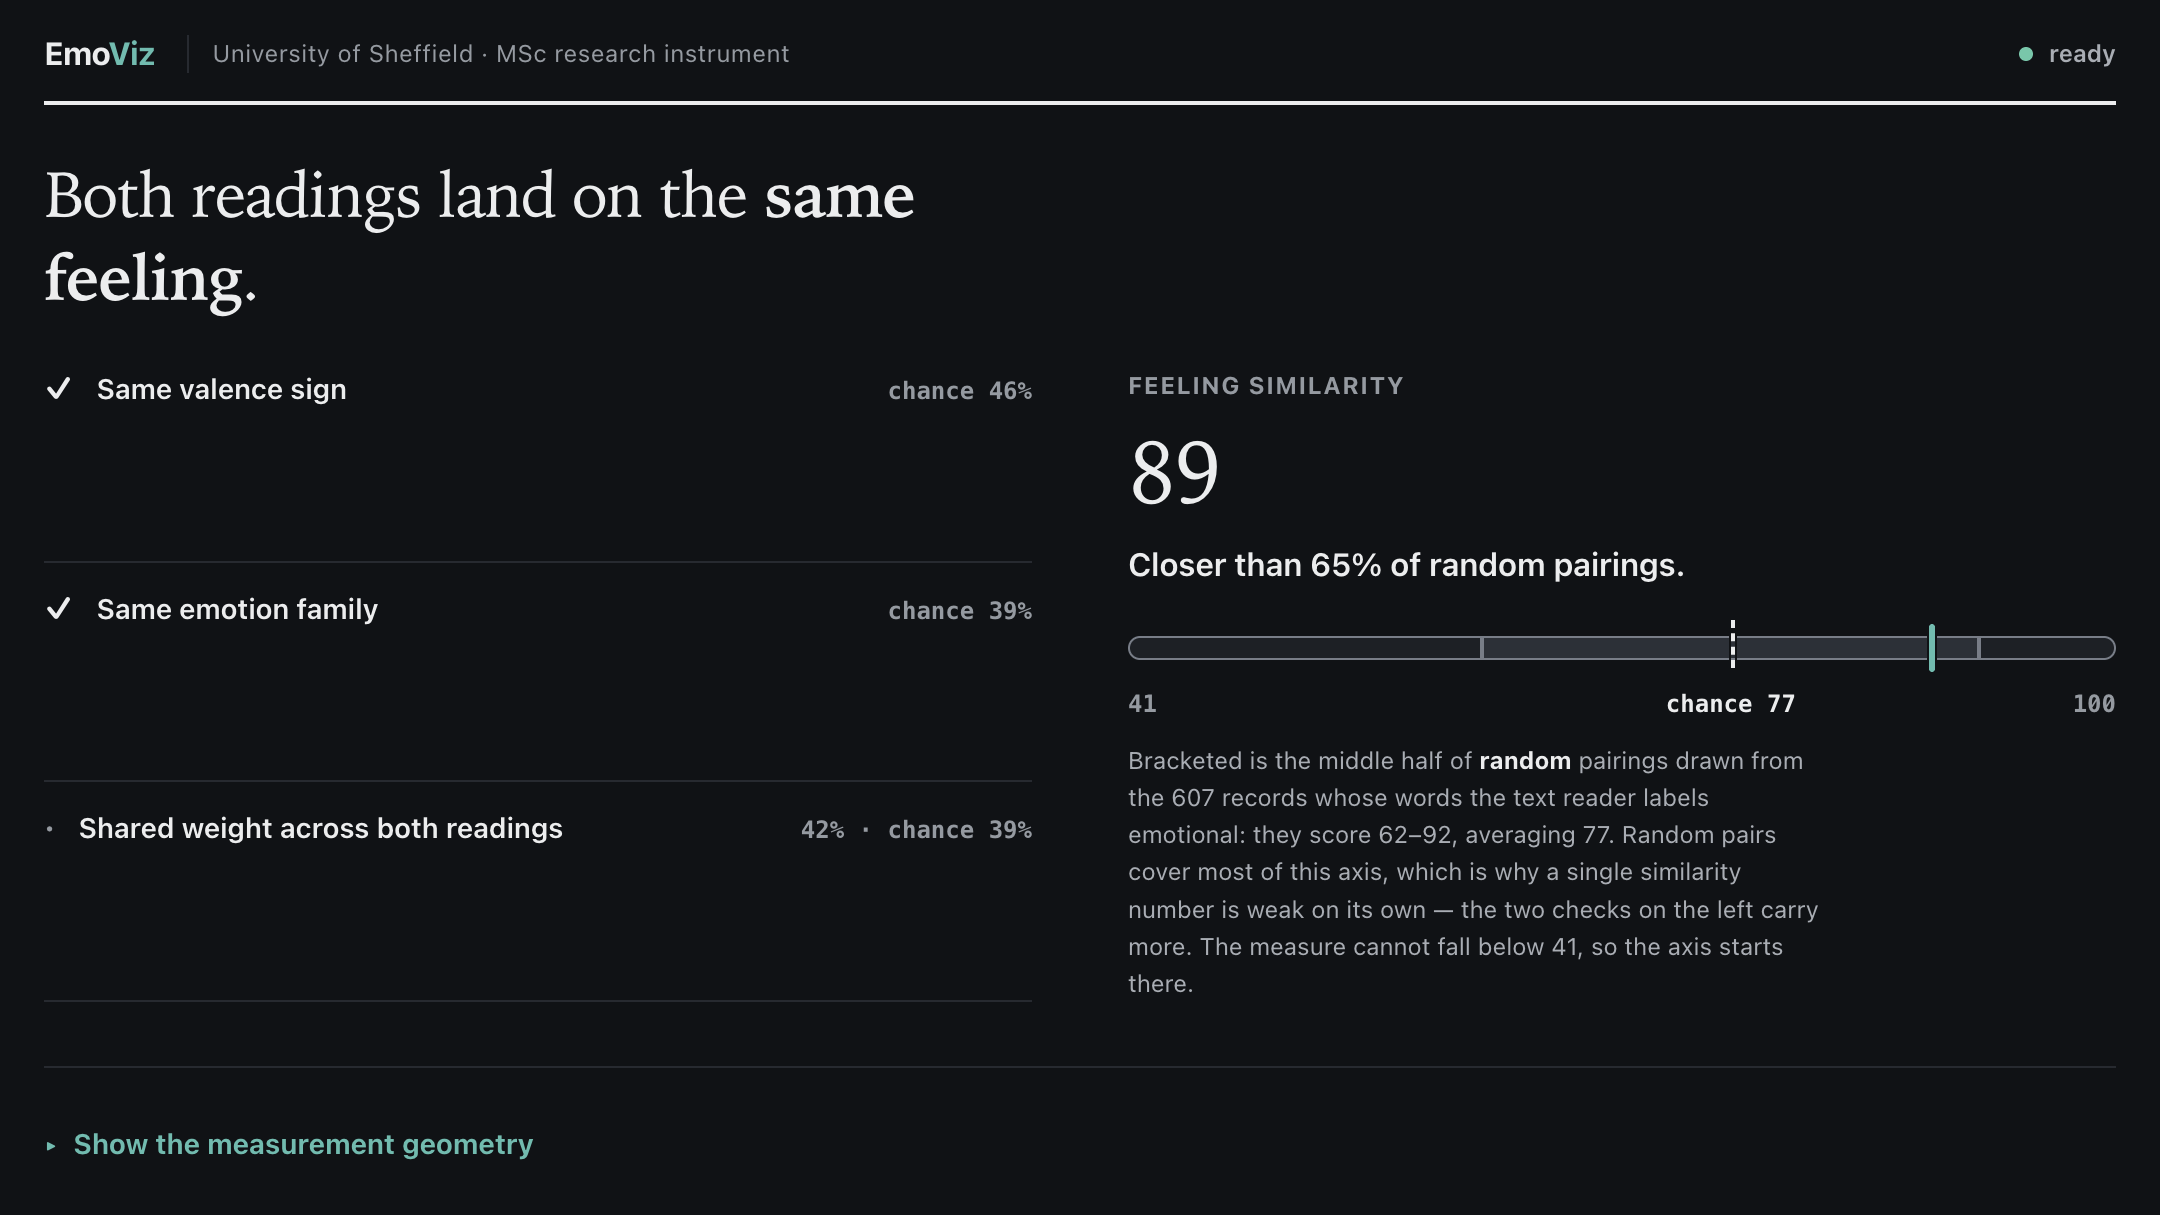
\includegraphics[width=\textwidth]{demo_screenshot}
\caption{The demonstrator's verdict after running record 63, ``super tired'', through the live models. Valence sign and family are reported first, each beside the chance level for that measure, and the third row gives the top-3 overlap. Valence--arousal similarity is not scored as a check but placed on its own axis on the right: the axis starts at its floor of 41, the shaded bracket is the middle half of the random pairings, the dashed mark is their mean and the solid mark is this record.}
\label{fig:demo}
\end{figure}

\section{Reproducibility and testing}
\label{sec:method-repro}

The environment is pinned in \texttt{requirements.txt}, Python 3.12 with PyTorch 2.13 and Transformers 5.14, on Apple silicon in float16, with about 3.5~GB of model downloads on first use. Every random process is seeded. Model outputs are cached record by record, the pipeline checkpoints to a JSONL file after each record so that a crash resumes where it stopped, and every stage after the pipeline reruns in seconds. Direct CLIP's readings are frozen in a file.

A single module, \texttt{emoviz/metrics.py}, defines each measure, each constant, the split rule and the null exactly once, and the scripts import from it, so a formula has nowhere to drift. Before it existed, two scripts had their own overlap formulas. They differed slightly. The difference changed no result on this data.

Testing has two layers. The first, \texttt{test.sh}, is a shell smoke suite: it verifies the environment, checks that the corpus and the cached outputs are intact, runs the redaction audit, runs each analysis script and requires a clean exit, pushes three fresh images through the live pipeline, and builds the figures, and any failure gives a non-zero exit. The second, \texttt{test\_numeric.py}, pins the headline numbers, comparing each one quoted in the text with the JSON value it comes from, to a stated tolerance, and it also unit-tests the measures themselves, the 0.412 floor, symmetry, overlap bounds and scale invariance, the sign map and the face rule. Figures come from \texttt{make\_figures.py} and the tables and macros from \texttt{export\_tex.py}, both reading the same JSON, so no result in this document was typed by hand.

The tests also have a limit. None of them compares a model's answer with a person's judgement. The completion figure, every one of the \nTotal{} images run through without an unhandled error, says that the code did not crash and nothing about whether its answers are any good, and a person enters the chain at one point only, the single-coder check. Appendix~\ref{app:repro} has the file list and the run order.
